\chapter{Locality Optimization for traversal-based Queries}\label{\positionnumber}
\section{Locality}\label{\positionnumber}
    The memory hierarchy tries to unify the strengths of fast, low capacity memory --- caches (SRAM) ---, with slower but larger memory --- main memory (DRAM), with orders of magnitude slower but orders of magnitude larger memory --- disks (HDD) and more recently flash memory (SSD, SD-Cards).
    Nevertheless, how can this work? 
    Given that only a tiny fraction of fast memory is available to hold the necessary parts, while additional loads of data are transferred in time --- ``desirably fast enough''.
    
    The fundamental principle for the memory hierarchy to work is called \textit{locality of reference} in the literature~\autocite{jacob2010memory, tanenbaum2015modern}. 
    This principle expresses that most programs do not access their address space uniformly or randomly but rather tend to access small subsets of all addresses in certain time intervals, depending on the program state.
    Locality can be approached in two ways~\autocite{denning2006locality}: 
    
    \begin{itemize}
     \item \textit{Temporal locality} refers to the number of other references between two accesses of the same memory location. 
     \item \textit{Spatial locality} refers to the number of accesses and the radius of the neighborhood that is accessed in several steps.
    \end{itemize}
    
    If the same location is accessed multiple times in a short amount of time, the temporal locality is high.
    Thus temporal locality can be measured using reference frequencies.
    From a Bayesian point of view, one can say that temporal locality is the probability of an object being re-referenced after the first usage~\autocite{gupta2013locality}. 
    \[ P (X_{t + \Delta} = A | X_t = A) \]
    $X_t$ is the reference at time step $t$, $A$ is an address, and $\Delta$ is a parameter, which depends not only on the system specifications (like the CPU and memory clock) also on the program and the scale of interest.
    
    If a small range of addresses is accessed very often, then spatial locality is high.
    If the range is limited to one address, then spatial locality is equivalent to temporal locality. Thus temporal locality is a particular case of temporal locality~\autocite{gupta2013locality}.
    With $\varepsilon$ a radius we can characterize spatial locality by:
    \[ P(X_{t + \Delta} = A \pm \varepsilon | X_t = A) \]
    Spatial locality is thus a function of time $\Delta$ and neighborhood range $\varepsilon$. 
    
    Several components profile the memory usage to leverage these concepts.
    In the memory hierarchy, all on and off-chip caches (i.e., SRAM) are handled by hardware~\autocite{jacob2010memory}.
    
    At the main memory level (DRAM), the operating system manages what is fetched, buffered, and evicted from disk to main memory. 
    The optimal buffering strategy is to load what is needed before its usage and evict the objects whose usage is furthest in the future~\autocite{tanenbaum2015modern}. 
    
    The best approximation to the optimal strategy is the least recently used algorithm when it comes to eviction. 
    It aims to keep things in memory that has the highest chance to exhibit temporal locality.
    The things in memory that have not been referenced for the longest time have a lower chance to be temporally local in the future~\autocite{silberschatz2006operating}.
    Put differently \textit{caches and buffers exploit temporal locality}.
    
    As this information is not available in general, objects are loaded when referenced, often with additional addresses that are hoped to be needed, too --- this is called prefetch or predictive fetching~\autocite{stallings2012operating, jacob2010memory}. 
    Prefetch tries to exploit spatial locality. Several components try to exploit this:
    \begin{itemize}
     \item Compiler-generated prefetches: 
     The compiler knows what addresses the program accesses in which sequence and tries to minimize the time spent waiting for IO. 
     We call this relocation instruction scheduling~\autocite{aho1986compilers}. 
     Other compiler-generated heuristics are applied, e.g., in domain-specific compilers, like in the TVM compiler for neural networks~\autocite{chen2018tvm}.
     
     \item The operating system may use specialized data structures and algorithms to estimate if prefetching should be done, based on the previous accesses. 
     An example is the ``spatial look-ahead'' algorithm by Baier and Sager~\autocite{jacob2010memory, baier1976dynamic}, but there exist many more e.g. \autocite{joseph1999prefetching, griffioen1994reducing, kroeger1997exploring, cooksey2002stateless}. 
     Most of these methods can find correlations between addresses and their neighborhood, file accesses, and pointed-to objects.
     
     \item A unique role in the context of prefetches and spatial locality take databases. 
     These can predict content-based correlations, e.g., by knowing what table is queried in the case of relational databases, but can also augment data by using auxiliary data structures like indices. 
     The most remarkable capability in this context is to reorganize data based upon how it is queried.
     Relational databases store data in tables and often sort these tables based upon either a specific field (like the primary key) or a set of fields. 
     In combination with being able to analyze the query before executing, this sorting allows reordering the memory accesses, such that as many accesses as possible are sequential~\autocite{ramakrishnan2000database, silberschatz1997database}.
    \end{itemize}
    
    Spatial locality depends on how data is ordered:
    If semantically closely coupled data is spread out as wide as possible, the program or file of interest will hardly exhibit locality. 
    As an example consider a program with $n$ instructions, with logical addresses from $0, \dots, n-1$. 
    An inversion is a change of position of two lines $l_1, l_2$, such that the line that gets executed earlier $l_1$ has a higher address than one that gets executed later $l_2$.
    Such a program can maximally have $\frac{n (n-1)}{2}$ inversions. 
    If it has that many inversions, the program is laid out in the opposite direction, and the spatial locality would be similar to the original program.
    Thus let us assume only every second instruction is misplaced. 
    In effect, to execute the program, two pages must always remain in memory instead of one, and the radius of the neighborhood doubles.
    
    In short, the layout of the data or records in the address space --- on file or in memory --- is crucial to the concept of spatial locality. 
    Achieving optimal temporal locality is a matter of grouping and ordering data such that what is referenced together is in a neighborhood in terms of addressing.
    
          
\section{Problem Definition}\label{prob-def}
    The records of the graph need to be grouped and ordered to optimize spatial locality for traversal-based queries.
    Ultimately disk storage and IO is block-based, and disk access is page-based. 
    That is, the vertices and edges must be grouped into blocks.
    This aggregation can happen statically or dynamically. 
    We focus here on the static reordering.
    That is, the underlying data is stored only on request.
    
    \paragraph{Assumptions:}
    In the remainder of this thesis, we are assuming that the graph is represented in the property graph model Section~\ref{prop-graph-model} and uses incidence lists (see Section~\ref{inci}) as the storage schema. 
    We are not taking properties, labels, and relationship types into account.
    We are focusing on spatial locality here; that is, the page replacement algorithm is fixed but arbitrary.
    Finally, in the remainder of the thesis, when talking about traversal-based queries, we mean all queries described in Section~\ref{queries}, but the random walk.
    
    \paragraph{Problem Definition:} Given a graph $G$, logical block size $b$, page size $p$. \\
    Desired is 
    \begin{enumerate}
     \item A partition of $G$ into blocks of vertex records $V_i$ and $E_i$ relationship records, 
     \item orderings or permutations $\pi_v, \pi_e$ of the blocks of vertex and edge records $V_i, E_i$,
     \item a reordering of the incidence list pointers
    \end{enumerate}
    such that spatial locality is as high as possible for traversal-based queries.
    
    As partitioning a graph optimally~\autocite{andreev2006balanced}, as well as finding an optimal linear arrangement~\autocite{garey1974some} are both NP-complete problems~\autocite{lewis1983computers}, we use the formulation ``as high as possible'' instead of optimal or maximal.
    
    To measure the spatial locality, we introduce two measures that are used in the evaluation chapter:
    \begin{enumerate}
     \item Number of block accesses.
     \item Number of non-consecutive block accesses.
    \end{enumerate}
    The first measure is to take the locality within a block into account:
This measure should be as small as possible when records that are accessed together are also stored together.
    The second measure takes the order of the blocks into account: 
    If vertices and edges that are connected or ``close'' to each other are stored in adjacent blocks, they can be loaded with one sequential read.
    The second measure also considers how the traversal is executed in terms of pointer chasing concerning the incidence list.
    
    As we change the unit of access from addresses of records to blocks on a disk, the definition of locality needs to be adapted.
    Temporal locality is now based on blocks instead of addresses.
     \[ P (X_{t + \Delta} = B | X_t = B) \]
     Here we have a block $B$ instead of an address $A$. 
     If blocks are well-formed, the number of blocks that are accessed should decrease overall.
     This decrease occurs because these multiple elements that are accessed in a short period are stored in the same block instead of several. \\
     Spatial locality can be reformulated in the same sense:
      \[ P(X_{t + \Delta} = B \pm \varepsilon | X_t = B) \]
      With a well-suited ordering of the blocks, the probability that neighboring blocks are accessed should be increased.
      Finally, when the incidence list is ordered, the access to blocks should be in a monotone increasing block address sequence. 
      Thus, the access should be sequential, and thus the probability of accessing adjacent blocks increases as opposed to unordered access that jumps back and forth.
    
\section{Locality in Vertex, Edge and Incidence List Order}
  Why are these three criteria necessary? Why are there only two measurements for three criteria? \\
  Those questions will be explained in an example.
  Something that is of importance for the traversal --- but not as straightforward to see as anode and edge grouping and order --- is the pointers' order in the incidence list, as we are going to see.
  
  \begin{figure}[htp]
    \begin{center}
        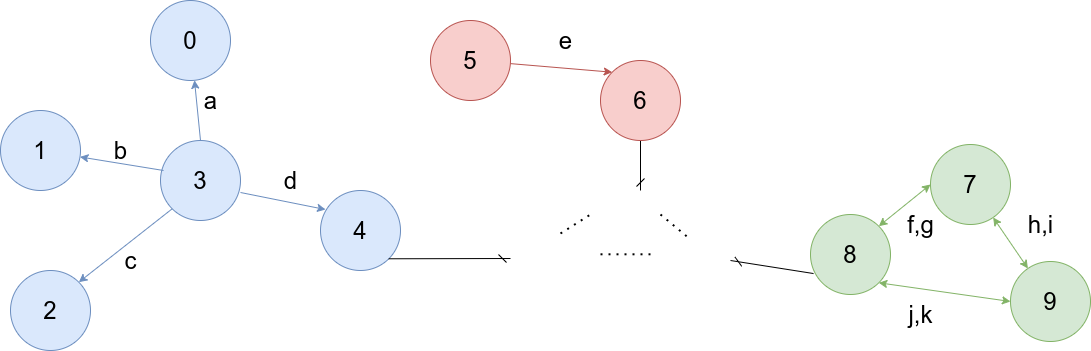
\includegraphics[keepaspectratio,height=0.3\textheight,width=\textwidth]{img/05-problem_def/example_graph.png}
    \end{center}
    \caption{Parts of a graph that is used in subsequent examples. Cut through edges mean edges to any non-visualized component of the graph. The dotted lines indicate, that other nodes and edges are between the three shown components.}
    \label{ex-gr}
  \end{figure}
  
  The graph used in the below example looks as shown in Figure~\ref{ex-gr}.
  We use a storage schema that is motivated by the one of Neo4J.
  Nodes and relationships are stored in separated files, the incidence list is stored in the edges' records, and the nodes contain a pointer to the head relationship of their incidence list each. 
  Moreover, we assume that we can only read sequentially if the blocks are adjacent.
  As this is a relatively short example for the sake of succinctness, things are just shown on a conceptual level. 
  We assume that three nodes or two relationships fit onto a disk block. 
  Realistically 8 to 16 nodes and 5 to 8 relationships fit on a 512-byte disk block. 
  An average graph in the Stanford network analysis platform graph dataset collection has thousands of nodes and edges. 
  Taking the californian road network graph as an example, the whole graph would take 
  \[ 1 965 206 \text{ nodes} \cdot 35 \text{ bytes per node} \cdot 512^{-1} \text{ bytes per block} = 134 341\text{ blocks}\] 
  to store all nodes and 
  \[2 766 607 \text{ relationships} \cdot 72 \text{ bytes per relationship} \cdot 512^{-1} \text{ bytes per block} = 389055\text{ blocks}\] 
  blocks to store the relationships in Neo4J.
  The principles shown below scale with the graph size, and for realistic assumptions, these conditions emerge.

  First, consider the split of vertices and edges into blocks in the upper half of Table~\ref{blocks}. 
  None of the vertices in the blocks are neighboring each other.
  Thus when traversing the graph, each step requires to load a block.
  The same is true for the edges: 
  None of the edges in the same block are connected to the same vertex. 
  Each edge causes a page fault and a load of another block(s).
  These additional block IOs may happen in current state-of-the-art graph databases like Neo4J. 
  The placement into blocks is currently by insertion order, thus depending on the input dataset's ordering. 
  In the lower half of Table~\ref{blocks}, vertices are grouped into blocks based on their neighborhood, and edges are grouped by the vertices to which they are connected.

  
     \begin{table}[htp]
     \centering
    \begin{tabular}[c]{|l|c|c|c|c|c|c|} \hline
    &&&&&&\\[-1em]
     node.db & \colorbox{blue!30}{0}, \colorbox{red!30}{5}, \colorbox{green!30}{7} & \colorbox{blue!30}{1}, \colorbox{blue!30}{4}, \colorbox{green!30}{9} & \colorbox{blue!30}{2}, \colorbox{red!30}{6}, \colorbox{green!30}{8} & \colorbox{blue!30}{3} &  & \\ \hline
     &&&&&&\\[-1em]
     edge.db & \colorbox{blue!30}{a}, \colorbox{green!30}{f} & \colorbox{blue!30}{b}, \colorbox{green!30}{g} & \colorbox{blue!30}{c}, \colorbox{green!30}{h} & \colorbox{blue!30}{d}, \colorbox{green!30}{i} & \colorbox{red!30}{e}, \colorbox{green!30}{j} & \colorbox{green!30}{k} \\  \hline
    \end{tabular}
    \vspace{0.5cm}
    
    \begin{tabular}{|l | c | c | c | c | c | c|} \hline
    &&&&&&\\[-1em]
     node.db & \colorbox{green!30}{7},\colorbox{green!30}{8}, \colorbox{green!30}{9} & \colorbox{blue!30}{0}, \colorbox{blue!30}{1}, \colorbox{blue!30}{3} & \colorbox{red!30}{6} & \colorbox{blue!30}{4}, \colorbox{blue!30}{2}, \colorbox{red!30}{5},  &  & \\ \hline
     &&&&&&\\[-1em]
     edge.db &  \colorbox{green!30}{f}, \colorbox{green!30}{h} & \colorbox{green!30}{g}, \colorbox{green!30}{k} & \colorbox{green!30}{i}, \colorbox{green!30}{j} & \colorbox{blue!30}{a}, \colorbox{blue!30}{b} & \colorbox{red!30}{e} & \colorbox{blue!30}{c}, \colorbox{blue!30}{d} \\ \hline
    \end{tabular}
  \caption{An example of suboptimal and improved record placement into blocks. 
  The block size is assumed to be only 3 vertex records and 2 node records respectively. 
  For larger block size, the same principle applies.}
   \label{blocks}
   \end{table}
    
  Next, Table~\ref{order} shows two different orderings of the blocks, this time with a focus on the edges only. 
  An edge is stored in the neighborhood of its source node in the upper table but far apart from its target node.
  Thus two single reads are required to go from one vertex over an edge to another vertex and retrieve its incident edges. 
  In the lower table, the blocks are adjacent, and one sequential read is enough to go from source to target and fetch the target's incidence list.
  
     \begin{table}[htp]
          \centering
    \begin{tabular}{|l | c | c | c | c | c | c|} \hline
    &&&&&&\\[-1em]
     edge.db &  \colorbox{green!30}{f}, \colorbox{green!30}{h}   & \colorbox{blue!30}{a}, \colorbox{blue!30}{b} & \colorbox{green!30}{i}, \colorbox{green!30}{j} & \colorbox{red!30}{e} & \colorbox{blue!30}{c}, \colorbox{blue!30}{d} & \colorbox{green!30}{g}, \colorbox{green!30}{k} \\ \hline
    \end{tabular}
    \vspace{0.5cm}
    
    \begin{tabular}{|l | c | c | c | c | c | c|}\hline
    &&&&&&\\[-1em]
     edge.db &  \colorbox{green!30}{f}, \colorbox{green!30}{h} & \colorbox{green!30}{g}, \colorbox{green!30}{k} & \colorbox{green!30}{i}, \colorbox{green!30}{j} & \colorbox{blue!30}{a}, \colorbox{blue!30}{b} & \colorbox{blue!30}{c}, \colorbox{blue!30}{d} & \colorbox{red!30}{e} \\ \hline
    \end{tabular}
      \caption{Suboptimal and improved block order.}
    \label{order}
       \end{table}
  
  Finally, consider the visualization of the incidence list of node 3, given the page placement in the upper part of Table~\ref{blocks} and Table~\ref{inc-ord}. 
  Theoretically, the only difference is the order in which the list points to the relationships. 
  We need to do four single reads when using the order given in the upper table in terms of traversed blocks. 
  The list may be loaded sequentially with one read operation instead of four single reads if we rearrange the pointers according to the lower table. 
  This phenomenon may also appear when the blocks are formed and ordered in an improved way, but only when scaling up to a larger neighborhood graph.
  An edge can be placed either near the other edges of the source or the target node.
When jumping back and forth, the impact will grow with the gaps between blocks in which those edges are stored.
  Finally, if the blocks are cached, this induces a higher load on the buffer manager, as more pages need to reside in memory simultaneously and as they are frequently re-referenced instead of being read once and evicted then.
  The higher the degree --- i.e., the length of the incidence list --- of the node, the more severe the effect.

\begin{table}[htp]
          \centering
    \begin{tabular}{|l | c | c | c | c |}\hline
     incidence list of node 3 &  c & a & d & b\\ \hline
    \end{tabular}
    \vspace{0.5cm}
    
    \begin{tabular}{|l | c | c | c | c |}\hline
     incidence list for node 3 &  a & b & c & d\\ \hline
    \end{tabular}
      \caption{Suboptimal and improved incidence list order.}
    \label{inc-ord}
\end{table}
